%%%%%%%%%%%%%%%%%%%%%%% file template.tex %%%%%%%%%%%%%%%%%%%%%%%%%
%
% This is a template file for Web of Conferences Journal
%
% Copy it to a new file with a new name and use it as the basis
% for your article
%
%%%%%%%%%%%%%%%%%%%%%%%%%% EDP Science %%%%%%%%%%%%%%%%%%%%%%%%%%%%
%
%%%\documentclass[option]{webofc}
%%% "twocolumn" for typesetting an article in two columns format (default one column)
%
\documentclass{webofc}
\usepackage[varg]{txfonts}   % Web of Conferences font
%
% Put here some packages required or/and some personal commands
%
%
\usepackage{hyperref}
\hypersetup{
    colorlinks=true,
    linkcolor=blue,
    urlcolor=cyan,
}
\usepackage{wrapfig}
\usepackage{tabularx}
\usepackage{svg}
\usepackage{natbib}
\usepackage{caption}
\captionsetup[figure]{font=small}
\usepackage{subcaption}
\usepackage{xcolor}

\definecolor{amethyst}{rgb}{0.6, 0.4, 0.8}
\definecolor{asparagus}{rgb}{0.53, 0.66, 0.42}
\definecolor{darkseagreen}{rgb}{0.56, 0.74, 0.56}
\definecolor{carolinablue}{rgb}{0.6, 0.73, 0.89}
\definecolor{beige}{rgb}{0.80, 0.78, 0.63}
\definecolor{fluorescentorange}{rgb}{.90, 0.65, 0.0}

\newenvironment{conditions}
  {\par\vspace{\abovedisplayskip}\noindent\begin{tabular}{>{$}l<{$} @{${}={}$} l}}
  {\end{tabular}\par\vspace{\belowdisplayskip}}

\begin{document}
%\title{CERN's 1000 Drupal Websites Move to Kubernetes}
\title{Building a Kubernetes infrastructure for CERN's Content Management Systems}
% NOTE: Drupal is probably not a relevant keyword for our audience to be in the title.
\author{\firstname{Konstantinos} \lastname{Samaras-Tsakiris}\inst{1}\fnsep\thanks{\email{konstantinos.samaras-tsakiris@cern.ch}} \and
        \firstname{Rajula} \lastname{Vineet Reddy}\inst{1}\fnsep \and
        \firstname{Francisco} \lastname{Borges Aurindo Barros}\inst{1,2}\fnsep \and
        \firstname{Eduardo} \lastname{Alvarez Fernandez}\inst{1}\fnsep \and
        \firstname{Andreas} \lastname{Wagner}\inst{1}
        % etc.
}

\institute{CERN \and Instituto Superior Técnico}

\abstract{%
The infrastructure behind \href{https://home.cern}{home.cern} and 1000 other Drupal websites serves more than 15,000 unique visitors daily.
To best serve the site owners, a small engineering team needs development speed to adapt to their evolving needs and operational velocity to troubleshoot emerging problems rapidly.
We designed a new Web Frameworks platform by extending Kubernetes to replace the ageing physical infrastructure and reduce the dependency on homebrew components.

The new platform is modular, built around standard components and thus less complex to operate.
Some requirements are covered solely by upstream open source projects, 
whereas others by components shared across CERN's web hosting platforms.
We leverage the \href{https://sdk.operatorframework.io/docs/}{Operator framework} and the Kubernetes API
to get observability, policy enforcement, access control and auditing, and high availability for free.
Thanks to containers and namespaces, websites are isolated.
This isolation clarifies security boundaries and minimizes attack surface, while empowering site owners.

In this work we present the new system's open-source design contrasted with the one it replaces, demonstrating how we drastically reduced our technical debt.
}
%
\vspace{-4.4em}
\maketitle
\vspace{-0.6em}
%
\section{Introduction}
\label{intro}
Google rewrites most of their software every few years \cite{henderson_software_2020}.
This surprising activity consumes a large fraction of their resources each year!
And yet, they consider it crucial to their agility and long-term success, because software requirements change as technologies evolve -- and with them, user expectations.
This practice typically reduces unnecessary complexity in each iteration,
and transfers knowledge into the new generation of engineers.

All these factors apply as much to CERN as they apply to Google.
Despite the much slower pace at which services evolve, CERN lives in the same dynamic technological environment.
Without a constant input of effort our software falls behind and fails to address modern expectations
of features and aspects such as security, high availability, portability and isolation.
At the same time unnecessary complexity accumulates:
yesterday's custom solutions can often be replaced with new upstream components,
the product of continuous standardization of solutions to problems that affect entire industries.

The increasing divergence between the original requirements the specified a piece of software and present requirements
results in \emph{technical debt} \cite{fairbanks_ur-technical_2020}.
The main purpose of this work is to pay back technical debt in CERN's Content Management Systems by modernizing the software architecture
and making the service more secure and flexible (see section \ref{sec-web-frameworks}).


\subsection{Why Kubernetes?}

Kubernetes is for cloud native applications an extension of what the operating system is for traditional applications.
It is becoming the de facto standard for Platform as a Service \cite{kaviani_towards_2019}, abstracting computational infrastructure and standardizing deployment,
so that an application can run unmodified on sites across the globe.
Scientific applications are routinely deployed on Kubernetes \cite{banek_why_2019, hariri_batch_2018, yuan_bioinformatics_2020},
and even HPC use cases are being investigated \cite{beltre_enabling_2019}.

At CERN the uptake is also evident.
CERN IT has integrated Kubernetes in the Cloud Infrastructure and allows instant provisioning of new clusters.
The ATLAS experiment is evaluating the replacement of all Grid computing services with Kubernetes clusters \cite{megino_using_2020}.
The Batch service, consisting of the largest portion of offline computational workloads at CERN, is prototyping a Kubernetes platform \cite{alvarez_managing_2020}.
REANA, a system for Reproducible Analyses, is targeting Kubernetes as a main execution backend \cite{simko_reana_2019}.

Many of these use cases are attracted by the promise of development velocity:
rapidly shipping features, while maintaining highly available services \cite{hightower_kubernetes_2017}.
A key element is to expand the pieces of a software stack that are immutable and versioned, declaratively configured, and self-healing.

\subsubsection*{Operator pattern}
\label{sec-operators}

The Web Frameworks use case is not only about using Kubernetes as a deployment vehicle.
Since we develop platforms and are concerned with their operational characteristics,
we extend Kubernetes with custom APIs and controllers, building infrastructure management applications that are part of Kubernetes.
Our applications range from integrating with other CERN systems to providing website management APIs and automating operations.

But what is included in the task of managing websites?
The infrastructure, seen as an application, needs to have a concept of a website and let users define the website they need: its name, the technology, parameters, etc.
Once a website is specified, the infrastructure needs to ensure that the website is automatically provisioned and set up.
More than just a server, this task might include setting up storage and database, and integration with external CERN systems.
After that, it needs to ensure that every component stays healthy and synchronized, propagating changes as requested by the user to every part.

In many cases, the solution has two components: a custom Kubernetes API and a controller that watches the API and ensures certain conditions.
This pattern is called \emph{Operator}, because it uses Kubernetes primitives to automate high-level operational workflows specific to the website technology.

\subsection{What is Drupal?}
\label{what-is-drupal}

Drupal is an open-source \emph{Content Management System} (CMS): a tool for site builders to organize and deliver content to their website visitors.
It's used in 10\% of the top-10k websites with the highest traffic \cite{builtwith_pty_ltd_open_nodate,q-success_di_gelbmann_gmbh_wordpress_nodate}.

The market leader in Drupal's niche is the CMS WordPress \cite{builtwith_pty_ltd_open_nodate}.
Drupal is often contrasted with it and, according to UX surveys conducted by a Drupal-focused company, seems to offer a complicated start for beginner users,
but a powerful experience for experts \cite{buytaert_state_nodate}.

Drupal is frequently embraced as an open source community-driven project, making it strategically attractive for \emph{enterprise sustainability} \cite{cern_geneva_real_2019}.
Use cases range from simple blogs to professional newspaper publishing, from enterprise presentation to e-commerce, across government and private sector entities \cite{drupal_community_explore_nodate}.
A frequently cited feature is the flexibility with which it adapts to bespoke requirements, while scaling to large amounts of content.

\subsubsection*{Drupal at CERN}
\label{drupal-at-cern}

Who can benefit from a dedicated infrastructure for CMS websites?
An organization that needs a dynamic Drupal environment, with high turnover of sites: universities, organizations comprising many departments and independent activities.
Drupal was selected as Content Management System due its active community and extensibility with contributed modules.
It has become the platform of choice for public outreach.

\subsection{Article structure}

Having laid down background information on the motivation, technologies and concepts used in this work, in the following sections we will describe:

\begin{tabular}{l|l}
    Section \ref{sec-drupalsvc} & \emph{What are the requirements} of Content Management as a Service at CERN?  \\
    Section \ref{sec-phys-infra} & What system \emph{currently} serves these requirements? \\
    Section \ref{sec-k8s-design} & What system did we design on Kubernetes \emph{to replace section \ref{sec-phys-infra}}? \\
    Section \ref{sec-experiment} & An experimental investigation of the new platform's efficiency \\
    Section \ref{sec-discussion} & Reflections on this work and plans for the future \\
\end{tabular}

%\section{What is required for Content Management as a Service?}
\section{Requirements for Content Management as a Service}
\label{sec-drupalsvc}
The service supports website admins to host and administer Drupal websites directed to the grand public,
such as experiment or departmental central websites.
Some of the most popular sites based on this service are \href{https://home.cern/}{home.cern}, \href{https://atlas.cern}{atlas.cern},
\href{https://cms.cern}{cms.cern}, \href{https://careers.cern}{careers.cern} and \href{https://visit.cern}{visit.cern}.
They form CERN's main outreach channel and are critical for the Organization's reputation.

Users of the service range across a wide spectrum of different professional profiles,
and it's quite common that the responsibility of site building at CERN falls on administrative personnel, or personnel with little technical background in web technologies.
This in turn shapes the kind of service we have to provide; it is, for example, impractical to rely on developer-centric workflows, like GitOps and CLI tools.
A small fraction of our user base, however, indeed have web development experience.

The consequence is that the Content Management service has a dual mission:
\begin{enumerate}
    \item to ensure the \emph{high availability} and performance of these communication channels
    \item to make site building and administration accessible to a wide-ranging user base, while remaining extensible for websites needing special features
\end{enumerate}

%This work describes an infrastructure project that focuses on furthering the \emph{first mission}, without sacrificing the second.
%Ideally, the changes should be almost transparent for non-technical site administrators, while enabling previously unavailable best-practices workflows for technical users.

\subsubsection*{Control vs. customization}

%All websites on the infrastructure are running the same Drupal distribution in a "multi-site" configuration, as will be explained in section \ref{sec-phys-infra}.
%The distribution consists of an upstream Drupal version with a few patches for the CERN environment, plus a curated set of "central" modules.
Curating the Drupal distribution, and critically, the application of \emph{security updates}, is the responsibility of the infrastructure team.
However, many websites need extra features and Drupal was selected exactly \hyperref[drupal-at-cern]{because of its extensibility}.
Website admins should be able to use community modules, thereby extending Drupal specifically for their website -- and assuming limited responsibility to keep custom code secure.

\subsection{Load characteristics}
\label{sec-load}

\href{https://home.cern/}{home.cern} is the most popular website at CERN, as shown in figure \ref{fig-drp-top10-cip}.
Out of \emph{1043} Drupal websites currently hosted, it alone serves 32\% of monthly unique visitors.
The top 10 websites together serve 79\% of all unique visitors, leaving only 1/5 of them headed for the other 1033 websites.
This is an intrinsic characteristic of the service load, which is heavily skewed towards a very small number of critical websites.

\begin{figure}[t]
    \centering
    \vspace{-3em}
    \begin{subfigure}[b]{.7\textwidth}
        \centering
        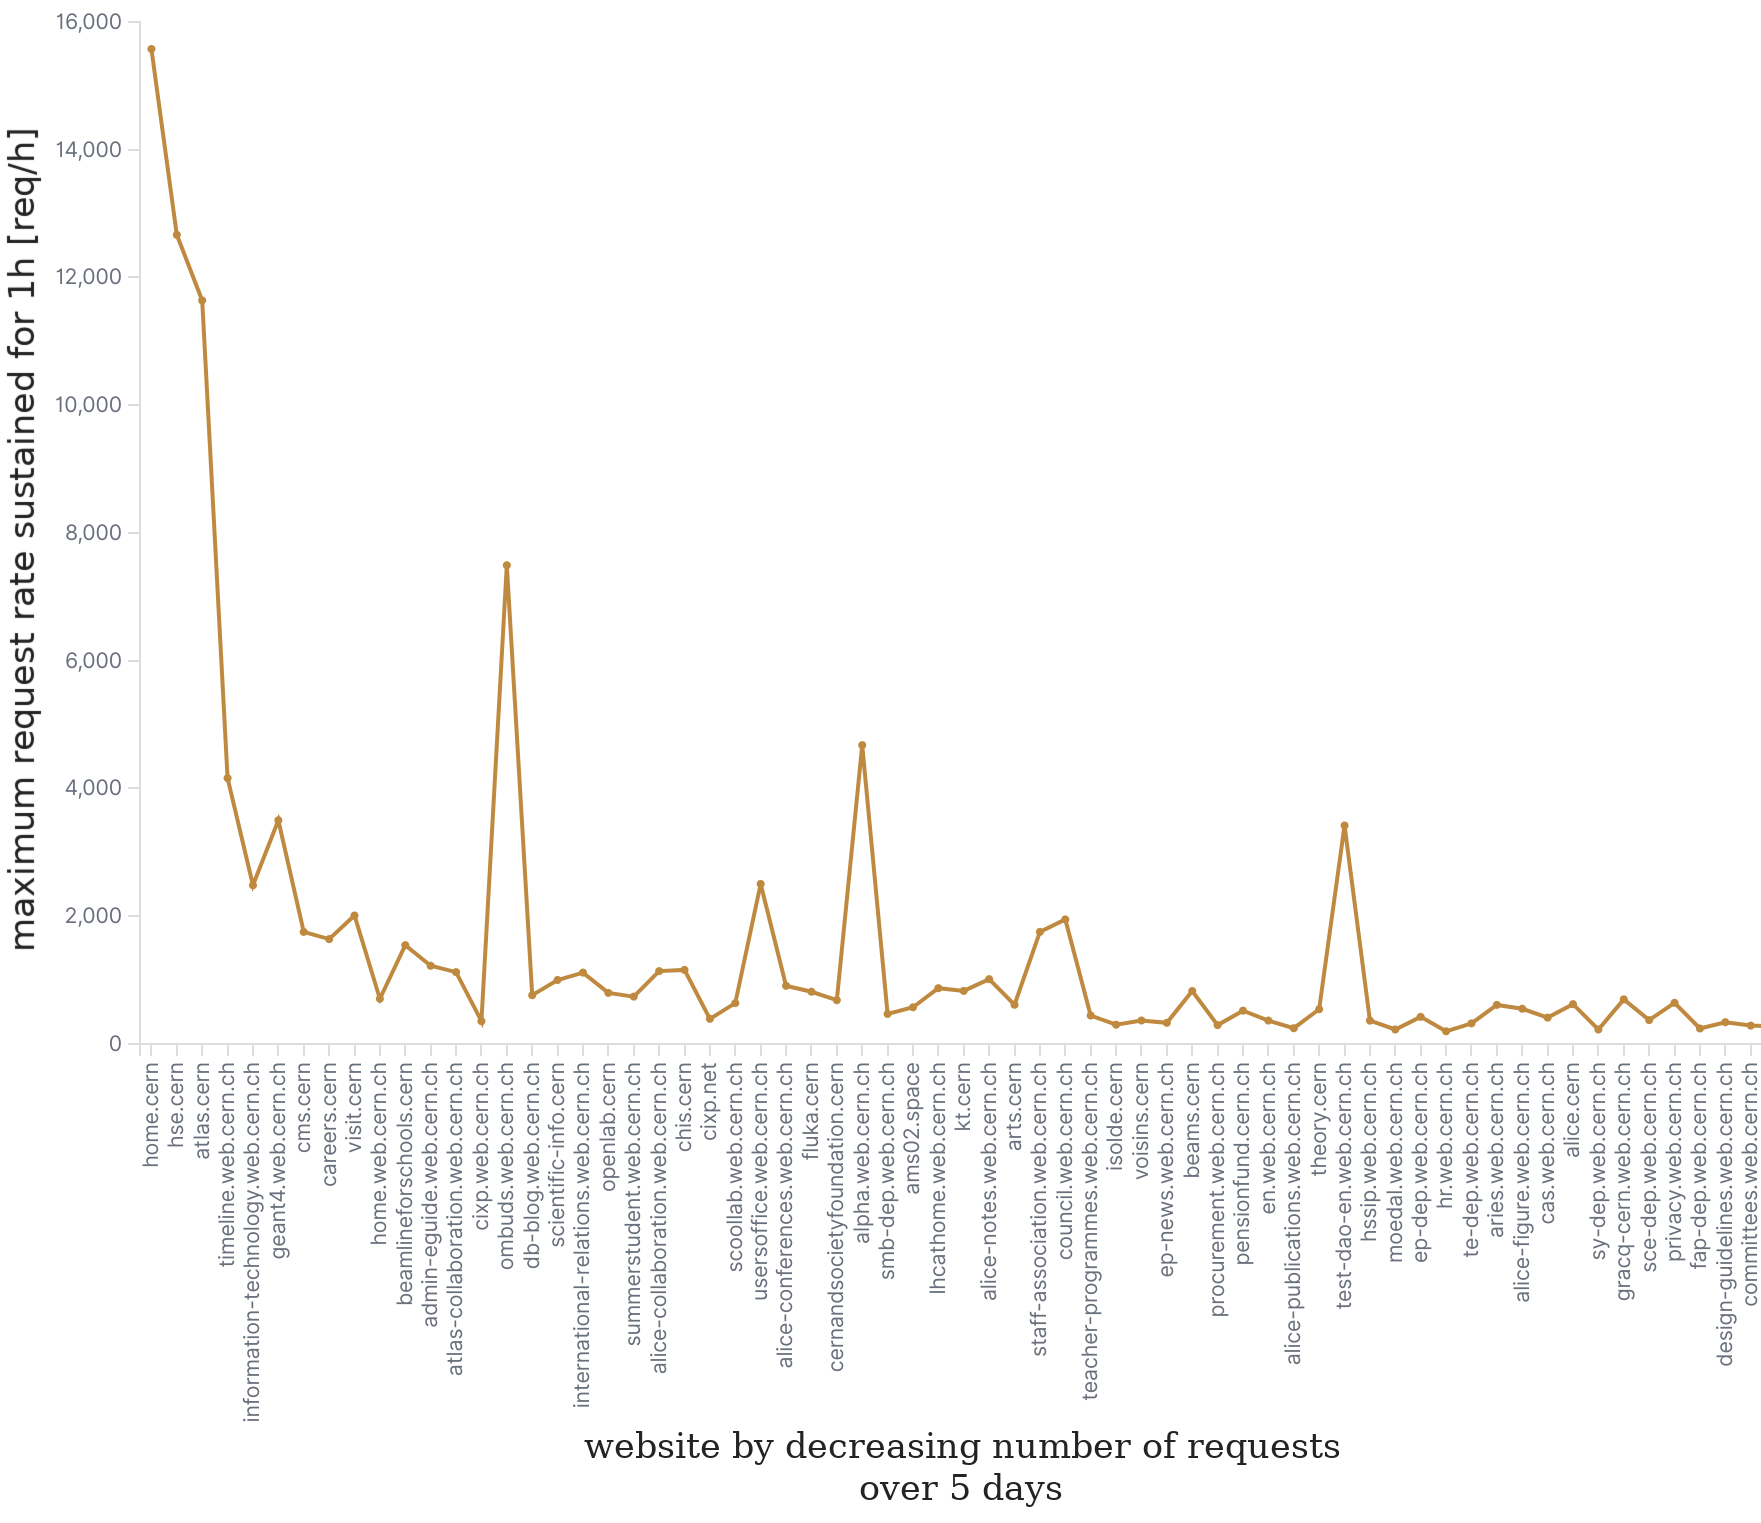
\includegraphics[width=\textwidth]{figures/website-bandwidth}
        \caption{\emph{Maximum sustained throughput for high traffic websites}.
          The maximum throughput of the highest traffic websites was recorded over a period of 5 days.
          The websites with the highest traffic also have the highest throughput, showing that sustained bursts of traffic are uncommon.}
        \label{fig:website_bandwidth}
    \end{subfigure}
    \hfill
    \begin{subfigure}[b]{.25\textwidth}
    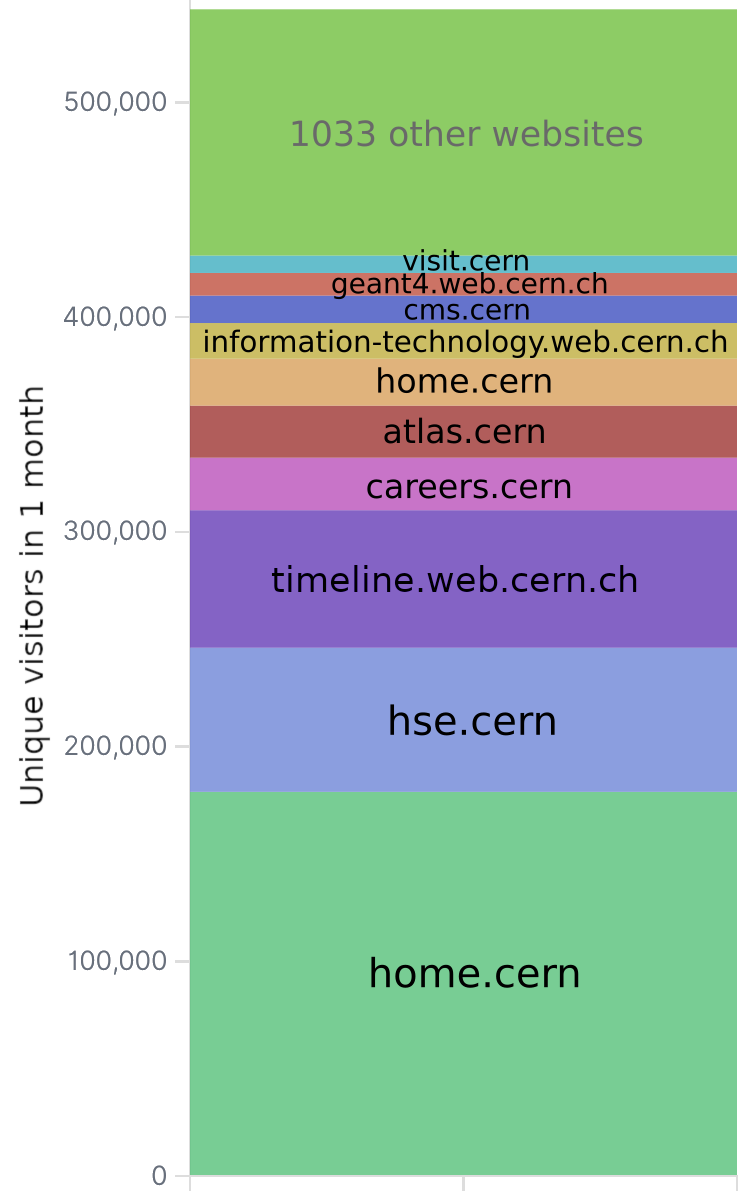
\includegraphics[width=\textwidth]{figures/drupal-top10-uniqClientIP.png}
    \caption{\emph{Public outreach}: 
        The top 10 most popular Drupal websites are shown.
        home.cern appears twice as \texttt{home.cern} and \texttt{home.web.cern.ch}.
        {\color{amethyst} \texttt{timeline.web.cern.ch}} has machine traffic.}
    \label{fig-drp-top10-cip}
    \end{subfigure}
    \vspace{-1.8em}
    \caption{Load characteristics}
    \vspace{-2em}
\end{figure}

Unique visitors over 1 month are taken as a measure of a site's popularity, or how much impact it has on the Organization's reputation,
but a measure more suitable to assess an infrastructure on is the rate of HTTP requests.
In section \ref{sec-experiment} we will describe an experiment on resource optimization in the Kubernetes infrastructure
by assigning websites to different Quality of Service classes.

The 10 websites with the highest traffic are the target of 60\% of all requests, and they have a high overlap with the most popular sites (fig. \ref{fig:website_bandwidth}).
The most popular websites therefore, apart from the highest availability guarantees, need also the highest throughput.

What sustained rate of requests should a website be able to handle with stable response time?
To better understand how the load impacts a single website (and therefore estimate the required hosting resources),
we performed the measurements of figure \ref{fig:website_bandwidth}.

These observations align with expectations and requirements: critical websites should be able to handle a throughput of 40 requests per second with stable response times.

\section{Current implementation}
\label{sec-phys-infra}
The infrastructure that currently serves the Drupal websites comprises 8 large physical Linux servers and a NAS shared filesystem.
It runs on CENTOS 7 and uses Puppet as configuration management system.
All servers run the same environment with Systemd services.
Major services are:
\begin{itemize}
    \item HAProxy load balancer: routes requests to worker nodes, with an affinity cookie
    \item Keepalived: implementation of floating IP for the load balancer
    \item Apache httpd: serves Drupal PHP code, WebDAV interface and a few additional PHP management applications
    \item php-fpm: maintains a pool of worker processes that generate Drupal content
\end{itemize}

\subsubsection*{Request journey}

When a request is made to a website on the infrastructure, eg home.cern, DNS resolves the name to the Drupal load balancer floating IP.
HAProxy then (hosted on 1 of the 8 servers) routes the request to one of the nodes.
Apache serves the request with Drupal PHP code. Drupal is configured to look up a directory for each site (multisite).
This flow can be seen in figure \ref{fig:drupal-physical-request-journey} together with the architecture.

Production websites respond to the load by spawning PHP workers, up to a maximum of 25.
A worker process is always listening for requests, even without load.
Test websites, on the other hand, spawn the first worker on demand and scale up to a maximum of 10 workers.
The PHP memory limit for every website is 512MB.

Websites have 2 data components: a directory and a database.
The directory lives on the NAS, shared among all servers.
The database is provided by an external dedicated service, Database on Demand (DBOD).

\begin{figure}[ht]
    \centering
    \hspace{-2em}
    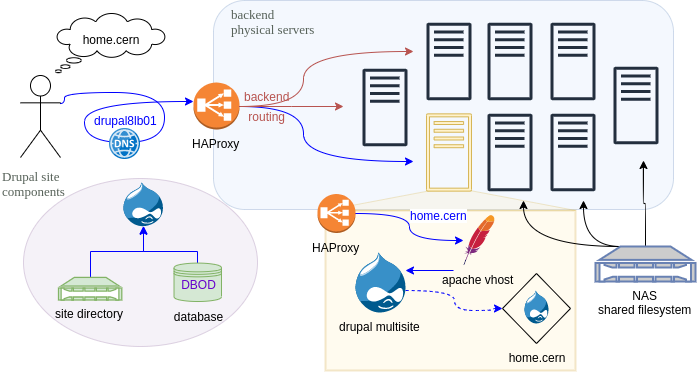
\includegraphics[width=\textwidth]{figures/drupal-physical-request-journey}
    \caption{\emph{Request journey in the physical infrastructure}.
    The current physical infrastructure consists of 8 physical Linux servers with a shared NAS filesystem.
    The {\color{blue} datapath} to access a site is shown in blue.
    The website's {\color{green} 2 data components}: a persistent directory on the NAS and a database on an external service (DBOD).
    }
    \label{fig:drupal-physical-request-journey}
\end{figure}

\subsubsection*{Website isolation}

Each website is assigned a Linux user.
Its directory is owned by it and not accessible by the users of other websites.
When Apache serves a request, it chroots the PHP process into the Drupal directory and sets the website's user.
This distinction provides a basic isolation mechanism.

Nevertheless, \emph{site isolation is relatively weak}.
We've never detected a cross-site security incident,
but there are no cgroup limits to resources, and not enough security layers to defend against privilege escalation exploits.
This is critical concern, given the vulnerability of CMS software \cite{shteiman_why_2014},
and the impact that defacing a high-traffic public site would have to CERN's reputation.

Furthermore, the website environment is inflexible.
All websites locked to the same Drupal version means massive, forced upgrade campaigns with little in the way of testing.
Better integration of testing and development environments is also lacking.

To top off the argument, the Drupal community is deprecating the multi-site functionality, % TODO ref
forcing us to adapt.

\subsection{Limitations of the current infrastructure}

Reiterating the discussion, these are the major limitations of the current infrastructure.
The Kubernetes infrastructure lifts all of them.

\begin{itemize}
    \item Hard to adjust resources, resulting in massive under-utilization
    \item Weak site isolation increases the risk of severe security incidents affecting multiple sites
    \item Inflexible website environment limits development \& testing workflows, makes upgrades cumbersome 
    \item \emph{Technical debt}: a lot of homebrew components built with legacy technologies specific to this system
\end{itemize}


\section{Pilot Kubernetes implementation}
\label{sec-k8s-design}
/subsection{Operator pattern}

https://www.openshift.com/learn/topics/operators

Kubernetes design principles, operators

\section{Measuring baseline resource requirements}
\label{sec-experiment}
\newenvironment{conditions}
  {\par\vspace{\abovedisplayskip}\noindent\begin{tabular}{>{$}l<{$} @{${}={}$} l}}
  {\end{tabular}\par\vspace{\belowdisplayskip}}

In order to deploy the new infrastructure, we first need an estimation of resources that Kubernetes will need in order to handle the same load as the physical infrastructure.
To make this estimation, we have stress tested each Quality of Service (QoS) and monitored the resources consumption. 

\subsection{Service level indicators}

In order to be able to answer each Quality of Service (QoS) differently, we have specified some metrics to help resource optimization without ignoring performance.
The defined metric that will be discussed here and will vary among each QoS is the capability of answering requests per second.

Using the physical infra as starting point (fig. \ref{fig:website_bandwidth}), we can observe the requests per second peaked on the most popular website, with around 16000 requests in an hour which averages on 4.4 requests per second.
We, therefore, have defined that there are three type of websites that translates into three types of Quality of Service:
\begin{itemize}
    \item \textbf{Critical} websites, these are the most popular and therefore the most important to have high capability of requests, the defined value is to handle 35 requests per second (Around 8 times the average on peak usage).
    \item \textbf{Standard} websites, these usually don't face as much traffic and therefore don't need to have high capability of requests, the defined value is to handle 10 requests per second. 
    \item \textbf{Test} websites, as in the name itself, these are used to test new features or add new content by website managers, and therefore are used by testers and developers, these type of websites only need to handle few requests, therefore the defined value is to handle 2 requests per second.
\end{itemize}

%- entire infra: 250 req/sec
%- critical website: 35 req/sec
%- standard website: 5-10 req/sec % TODO set final value
%- test website: 2 max threads

%- Find configuration that is able to handle specified req/sec load
%- Two Graphs (1 for critical and 1 normal), showing AVG response time plots + Request per second plots
%- See the Resources usage for each configuration
%- Make an estimation of total resources , note that critical websites will have $(MAX_LOAD) + 2(IDLE_LOAD)$ since they will have 3 pods

%Total number of Critical websites: 20
%Total number of Standard websites: 600
%Total number of Test websites: 500
%- Make an estimation of total infra resources ( sum to the estimation of total resources with openshift-* elements)

% #### Resources used in the physical infra:
% - Memory: 2TB
% - CPU: 512

\subsection{Stress test setup}

% (we have provioned websites and migrated data from the old infra)
To have a proper setup to test, we have migrated some websites with diversified content to the new infrastructure to observe how websites already hosted under the Physical infra perform on the Kubernetes infrastructure.

%To evaluate the behavior of our Kubernetes infrastructure, with the goal of analysing the new infrastructure's capability of answering the same needs with fewer resources, the following experiment was conducted.

%The following elements were required, 

The experiment has a dedicated Kubernetes cluster that deploys a custom tool based on \hyperlink{locust.io}{Locust} to make multiple requests to the targeted website on the new infrastructure. 
The simulation of requests is done by running multiple \hyperlink{https://kubernetes.io/docs/concepts/workloads/pods/}{Pods}, each containing multiple processes that will request URLs at random\footnote{It iterates urls through the website to discover all the URLs, and only after having all the URLs, it connects to one of them at random}.

\subsubsection{Stress load}
Multiple runs have been made with different configurations in order to find a suitable one for each QoS to process the desired requests per second with minimal resource consumption.

We observed that after a number of parallel users in the same pod, the users would get bottle-necked by Pod network constraints. So for our tests we observer that each Pod could have no more than 5 processes before network constraints would interfere.

%Important notes:
%- RAM consumption before first connection is ~11MiB, 500 to 600MiB after (even if no accesses are being done)
%- Time used for a stress run was decided to be 6min because it's enough to see the stabilized response time

\subsubsection{Measurements}

The following graph shows the average response time from the client's side as well the requests per second handled from the server side at the same time. 

The stress tests do a ramp up during the first minute, after which they maintain the stress load for more 9 minutes.
Thus, the total duration for each run is 10minutes, this value was considered enough to present the trend that would follow in a bigger time frame.

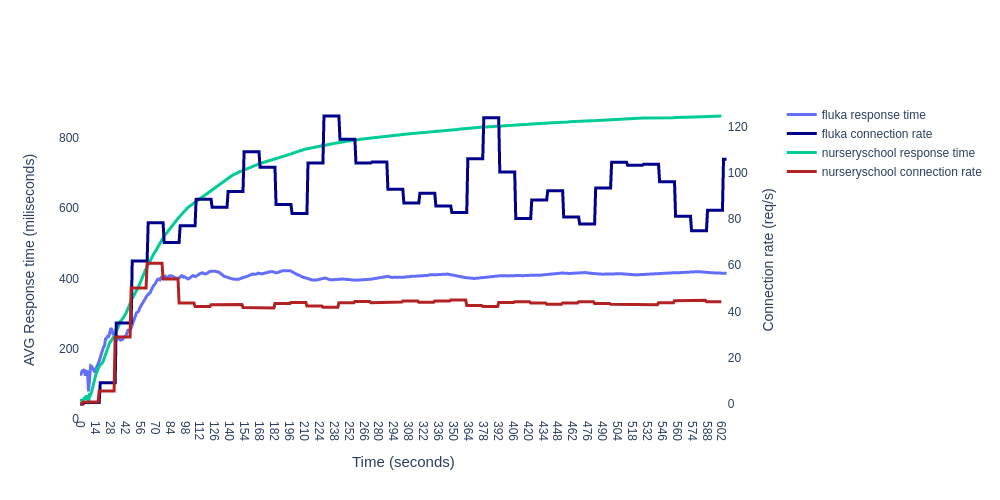
\includegraphics[width=400]{figures/experiment-figures/critical_run.png}

During this run, the resources consumption was also monitored, here we can see the usage for `nursery` and `fluka` websites respectively:

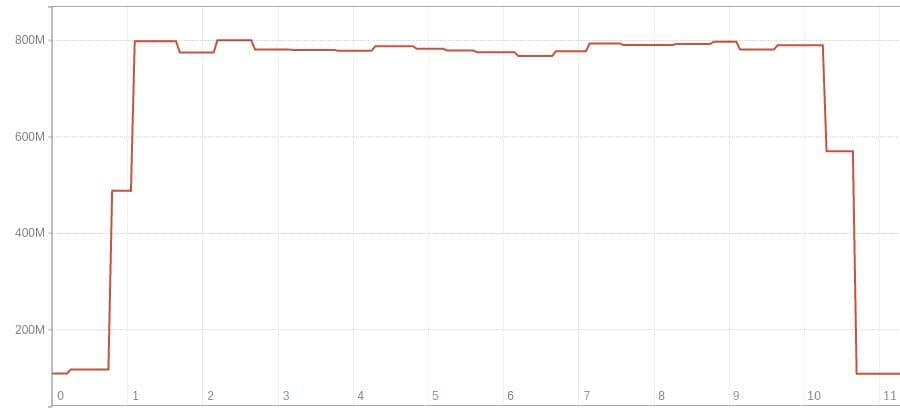
\includegraphics[width=\linewidth/2]{figures/experiment-figures/nursery_memory_usage.jpg}
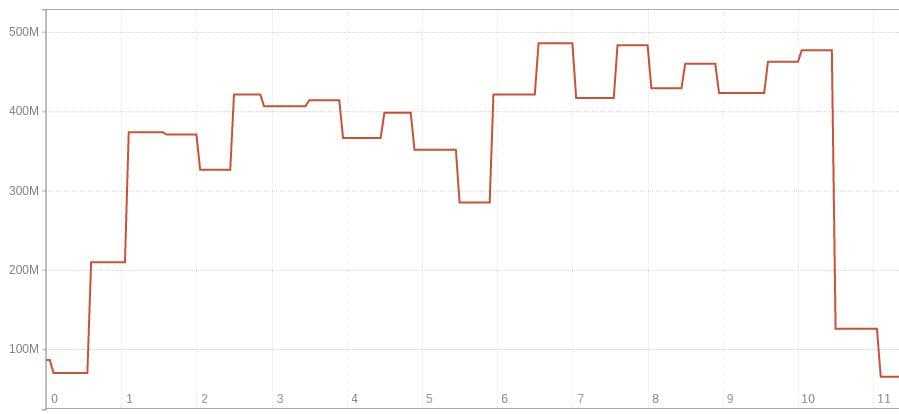
\includegraphics[width=\linewidth/2]{figures/experiment-figures/fluka_memory_usage.jpg}

The same experiment was conducted to the same websites with configurations based on the other QoS. 
The following tables show the highest response time under full stress and lowest requests per second for each QoS.

\begin{table}[!htb]
\centering
\parbox{.45\linewidth}{
\begin{tabular}{|l|ll|ll}
\cline{1-3}
\textbf{website} & \multicolumn{1}{l|}{\textbf{Stress (req/s)}} & \textbf{Response (ms)} &  &  \\ \cline{1-3}
nurseryschool    & 18                                           & 240                    &  &  \\ \cline{1-1}
fluka            & 48                                           & 103                    &  &  \\ \cline{1-3}
\end{tabular}
}
\hfill
\caption{Standard QoS values}
\parbox{.45\linewidth}
{\begin{tabular}{|l|ll|ll}
\cline{1-3}
\textbf{website} & \multicolumn{1}{l|}{\textbf{Stress (req/s)}} & \textbf{Response (ms)} &  &  \\ \cline{1-3}
nurseryschool    & 41  & 870   &  &  \\ \cline{1-1}
fluka            & 74  & 600   &  &  \\ \cline{1-3}
\end{tabular}
}
\caption{ Critical QoS values}
\end{table}





%Table \ref{tabel_of_resources}
\begin{table}[]
\centering
\label{tabel_of_resources}
\begin{tabular}{|l|ll|ll}
\cline{1-3}
\textbf{QoS} & \multicolumn{1}{l|}{\textbf{CPU}} & \textbf{RAM(MiB)} &  &  \\ \cline{1-3}
test         & 0.3                                & 104               &  &  \\ \cline{1-1}
standard     & 2.3                                & 257               &  &  \\ \cline{1-1}
critical     & 3  & 800               &  &  \\ \cline{1-3}
\end{tabular}
\caption{ Resources peak consumption per QoS.}
\end{table}
% Show that we have STABLE response times

\subsection{Results: resource provision}

Based on the results seen in measurements section, we can now make an estimation of resource provision for the new infrastructure based on the values retrieved.

For expected memory:
\[
\begin{array}{rcl}
TotalMem & = & C * L + 2* C * I + S * L + T * L \\
 & = & 20 * 960MiB + 20*104MiB + 600*257MiB + 500*200MiB \\
 & = & XYZ MiB = XYZGB
\end{array}
\]
Where:
\begin{conditions}
Expected Load  &  Max Seen load + 20\% overhead \\
 L     &  Expected Max Load for specific QoS website \\
 I     &  Expected Idle Load for specific QoS website \\   
 C     &  Total number of Critical Websites \\
 S     & Total number of Standard Websites \\
 T     & Total number of Test Websites \\
\end{conditions}

On the physical infrastructure we have provisioned 2TB of memory, on the new Kubernetes infrastructure we have a rough estimation on total memory used if all websites are under load is of about 443GB. The prediction expects to only have 22.15\% of the memory required in the physical infrastructure.


For expected cpu:
\[
\begin{array}{rcl}
TotalCPU & = & C * L + 2* C * I + S * L + T * L \\
 & = & 20 * 3VCpu + 2*0.01VCpu + 600* 1.6VCpu + 500* 1VCpu \\
 & = & FINALRESULT
\end{array}
\]




\section{Reflections}
\label{sec-discussion}
It is striking how big a difference it makes to discuss a design with 10 engineers rather than 3, and to have the peace of mind in case of emergency that many colleagues can take part.
This is the hidden benefit of sharing a common platform, which this team has already felt.
Especially in CERN's dynamic environment where the turnover of people is high, knowledge silos can be ill afforded.

The Pilot phase of this new infrastructure is still too immature to provide significant operational insights.
We fully expect a few minor adaptations of the presented design as we scale up to production, but the experiments of
section \ref{sec-experiment} reassure us that the infrastructure is functional and that modifications should be limited to the details.
On the other hand, all the limitations of the physical infrastructure of section \ref{sec-limitations} have been lifted.

The next big challenge will be the production migrations in Q2 2021.
Development is ongoing, including critical features for production.
It is important to keep them as transparent to the website admins as possible and minimize disruption.
From the power users however we expect the new features to receive a warm welcome and open new doors in their workflows.

\subsubsection*{Directions to explore}

Develop once, run everywhere is a yet-to-be materialized promise.
Plans for disaster recovery from a catastrophic failure of the CERN data center hinge on maintaining a public communications channel accessible.
With Kubernetes cluster federation, using Public Cloud resources as a safety net is conceivable.

We will explore adding WordPress as a Service to the same infrastructure.
Fundamentally, it should take no more than introducing a new build configuration.

The \href{https://landscape.cncf.io/}{CNCF landscape} provides a salient overview of industry-standard solutions that can take this project the proverbial extra "mile".
We plan to experiment with runtime security, root cause analysis, chaos engineering and serverless for the non-production environments.
Kubernetes turns a homebrew system into a cosmopolitan denizen of a brave new world of the Cloud.

\section*{Acknowledgements}

This work relies upon the contributions of all members of the Web Frameworks section of CERN's IT department,
especially those that designed and implemented the common components.
We thank specifically Alex Lossent, Ismael Posada Trobo, Joao Esteves Marcal, Iago Santos Pardo, Aleksandra Wardzinska, Michal Kolodziejski and Emmanouil Fokas.

\bibliography{references.bib}
\end{document}